% Input: 80 MSa/s * 32 bits = 2560 Mbit/s.
% UART: sensor-firmware/main/sensor_uart_downlink.c, 3000000 baud.
% SPI: controller-firmware/main/espargos_spi.h, SPI_MASTER_FREQ_13M
%      = 80 MHz / 6, single data lane.
% S31: high-speed USB 480 Mbit/s; Gigabit Ethernet 1000 Mbit/s.
% Pipe width = 42pt * sqrt(link rate / 2560); not a linear width scale.
% Build: pdflatex iq-bandwidth.tex; pdf2svg iq-bandwidth.pdf iq-bandwidth.svg
\documentclass[border=6pt]{standalone}
\usepackage{helvet}
\renewcommand{\familydefault}{\sfdefault}
\usepackage{tikz}
\usetikzlibrary{arrows.meta,calc}
\definecolor{accent}{HTML}{37C964}
\definecolor{surface}{HTML}{293135}
\definecolor{foreground}{HTML}{DEE2E6}
\definecolor{muted}{HTML}{ADB5BD}
\definecolor{outline}{HTML}{66757D}
\begin{document}
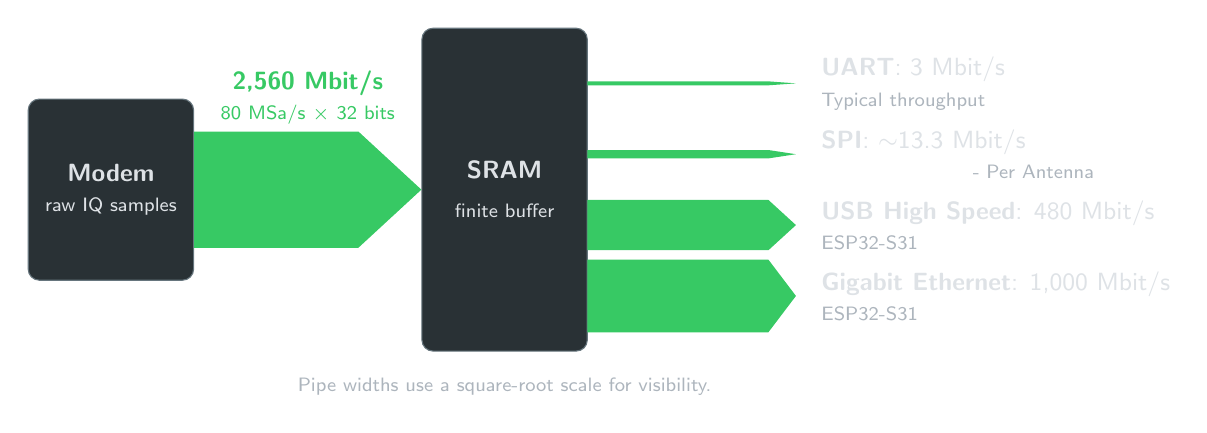
\begin{tikzpicture}[font=\sffamily\small, text=foreground,
  block/.style={draw=outline, fill=surface, rounded corners=4pt, align=center},
  label/.style={align=center, font=\scriptsize, text=muted}]
  \node[block, minimum width=2.1cm, minimum height=2.3cm] (modem) at (0,0)
    {\textbf{Modem}\\{\scriptsize raw IQ samples}};
  \node[block, minimum width=2.1cm, minimum height=4.1cm] (sram) at (5,0)
    {\textbf{SRAM}\\[3pt]{\scriptsize finite buffer}};

  % Single filled outline avoids seams from a thick stroke and arrowhead.
  \path[fill=accent]
    ($(modem.east)+(0,21pt)$)
    -- ($(sram.west)+(-8mm,21pt)$)
    -- (sram.west)
    -- ($(sram.west)+(-8mm,-21pt)$)
    -- ($(modem.east)+(0,-21pt)$) -- cycle;
  \node[align=center, text=accent] at (2.5,1.17)
    {\textbf{2,560 Mbit/s}\\{\scriptsize 80 MSa/s $\times$ 32 bits}};

  \foreach \y/\rate/\title/\note/\speed in {
    1.35/3/UART/Typical throughput/{3 Mbit/s},
    .45/13.333/SPI/{{\color{white}ESPARGOS One} - Per Antenna}/{\(\sim\)13.3 Mbit/s},
    -.45/480/USB High Speed/ESP32-S31/{480 Mbit/s},
    -1.35/1000/Gigabit Ethernet/ESP32-S31/{1,000 Mbit/s}} {
    \pgfmathsetmacro{\pipewidth}{42*sqrt(\rate/2560)}
    \pgfmathsetmacro{\halfwidth}{\pipewidth/2}
    \path[fill=accent]
      ($(6.05,\y)+(0,\halfwidth pt)$)
      -- ($(8.35,\y)+(0,\halfwidth pt)$)
      -- (8.7,\y)
      -- ($(8.35,\y)+(0,-\halfwidth pt)$)
      -- ($(6.05,\y)+(0,-\halfwidth pt)$) -- cycle;
    \node[anchor=west, align=left] at (8.9,\y)
      {\textbf{\title}: \speed\\{\scriptsize\color{muted}\note}};
  }
  \node[label] at (5,-2.5)
    {Pipe widths use a square-root scale for visibility.};
\end{tikzpicture}
\end{document}
